\documentclass[sigconf]{acmart}
% =============================================================================
% Template setup — participants normally do not edit this file.
% Author content belongs in main.tex; citations belong in main.bib.
% \documentclass lives in main.tex so Overleaf does not treat this file as root.
% =============================================================================


% --- Competition / non-ACM-submission friendly rights metadata -------------
\setcopyright{none}
\settopmatter{printacmref=false}
\acmConference[Kaggle Competition]{Filament Segmentation Challenge}{2026}{\href{https://www.kaggle.com/competitions/filament-segmentation-2026}{kaggle.com/competitions/filament-segmentation-2026}}
\acmBooktitle{Competition Report}
\acmDOI{}
\acmISBN{}


% --- Author guidance text --------------------------------------------------
% \guide{...} is gray italic while \guideStyletrue; omitted from the PDF if false.
% Flip the switch in main.tex after % =============================================================================
% Template setup — participants normally do not edit this file.
% Author content belongs in main.tex; citations belong in main.bib.
% \documentclass lives in main.tex so Overleaf does not treat this file as root.
% =============================================================================


% --- Competition / non-ACM-submission friendly rights metadata -------------
\setcopyright{none}
\settopmatter{printacmref=false}
\acmConference[Kaggle Competition]{Filament Segmentation Challenge}{2026}{\href{https://www.kaggle.com/competitions/filament-segmentation-2026}{kaggle.com/competitions/filament-segmentation-2026}}
\acmBooktitle{Competition Report}
\acmDOI{}
\acmISBN{}


% --- Author guidance text --------------------------------------------------
% \guide{...} is gray italic while \guideStyletrue; omitted from the PDF if false.
% Flip the switch in main.tex after % =============================================================================
% Template setup — participants normally do not edit this file.
% Author content belongs in main.tex; citations belong in main.bib.
% \documentclass lives in main.tex so Overleaf does not treat this file as root.
% =============================================================================


% --- Competition / non-ACM-submission friendly rights metadata -------------
\setcopyright{none}
\settopmatter{printacmref=false}
\acmConference[Kaggle Competition]{Filament Segmentation Challenge}{2026}{\href{https://www.kaggle.com/competitions/filament-segmentation-2026}{kaggle.com/competitions/filament-segmentation-2026}}
\acmBooktitle{Competition Report}
\acmDOI{}
\acmISBN{}


% --- Author guidance text --------------------------------------------------
% \guide{...} is gray italic while \guideStyletrue; omitted from the PDF if false.
% Flip the switch in main.tex after \input{preamble}.
%
% Do not use \guide{...} for \email{...}.
\usepackage{xcolor}
\newif\ifguideStyle
\guideStyletrue
\newcommand{\guide}[1]{%
  \ifguideStyle
    {\color{gray!65}\itshape #1}%
  \fi
}


% --- Math ------------------------------------------------------------------
% Do NOT load amssymb (or amsfonts): acmart already loads newtxmath, which
% defines the same symbols (e.g. \Bbbk) and causes a conflict on Overleaf.
% amsmath is already provided by acmart; mathtools extends it.
\usepackage{mathtools}


% --- Figures ---------------------------------------------------------------
% graphicx is already loaded by acmart
\usepackage{subcaption}


% --- Tables ----------------------------------------------------------------
% booktabs is already loaded by acmart
\usepackage{tabularx}
\usepackage{multirow}


% --- Bibliography style is set in main.tex (ACM-Reference-Format) ----------

.
%
% Do not use \guide{...} for \email{...}.
\usepackage{xcolor}
\newif\ifguideStyle
\guideStyletrue
\newcommand{\guide}[1]{%
  \ifguideStyle
    {\color{gray!65}\itshape #1}%
  \fi
}


% --- Math ------------------------------------------------------------------
% Do NOT load amssymb (or amsfonts): acmart already loads newtxmath, which
% defines the same symbols (e.g. \Bbbk) and causes a conflict on Overleaf.
% amsmath is already provided by acmart; mathtools extends it.
\usepackage{mathtools}


% --- Figures ---------------------------------------------------------------
% graphicx is already loaded by acmart
\usepackage{subcaption}


% --- Tables ----------------------------------------------------------------
% booktabs is already loaded by acmart
\usepackage{tabularx}
\usepackage{multirow}


% --- Bibliography style is set in main.tex (ACM-Reference-Format) ----------

.
%
% Do not use \guide{...} for \email{...}.
\usepackage{xcolor}
\newif\ifguideStyle
\guideStyletrue
\newcommand{\guide}[1]{%
  \ifguideStyle
    {\color{gray!65}\itshape #1}%
  \fi
}


% --- Math ------------------------------------------------------------------
% Do NOT load amssymb (or amsfonts): acmart already loads newtxmath, which
% defines the same symbols (e.g. \Bbbk) and causes a conflict on Overleaf.
% amsmath is already provided by acmart; mathtools extends it.
\usepackage{mathtools}


% --- Figures ---------------------------------------------------------------
% graphicx is already loaded by acmart
\usepackage{subcaption}


% --- Tables ----------------------------------------------------------------
% booktabs is already loaded by acmart
\usepackage{tabularx}
\usepackage{multirow}


% --- Bibliography style is set in main.tex (ACM-Reference-Format) ----------


\guideStylefalse
\setlength{\emergencystretch}{2em}
\begin{document}
\title{ThreadMask: full-resolution ridge refinement of learned filament masks}
\subtitle{A Solution to the Solar Filament Segmentation Challenge 2026}
\author{Jacek Adamek}
\affiliation{\country{Poland}}
\email{jacman1988@gmail.com}
\begin{abstract}
This report describes our solution to the Solar Filament Segmentation Challenge 2026, a Kaggle competition on automatic segmentation of solar filaments in GONG H-alpha observations. We combine a CPU pixel-forest baseline, learned component rejection and a new full-resolution ridge regressor. Across 146 development observations from 135 dates, local public-metric PQ changes from 0.276155 to 0.277402, false positives from 810 to 807, and thin annotation-level matches from 126/442 to 127/442. The additional 40-date comparison adds no thin matches and uncertainty intervals include zero. These are reused development results, not a new Kaggle score or independent evidence of improvement. The image-only candidate, unsuccessful alternatives and reproducible checks are documented without claiming a novel segmentation algorithm.
\end{abstract}
\maketitle
\noindent\textbf{Prepared update, 16 October 2026. Proposed competition update; not submitted.}
\section{Introduction}
This report goes over the details of our submitted solution to the Solar Filament Segmentation Challenge 2026 [1]. The challenge, launched on July 10, 2026, is organized by the Earth-Space AI Research (ESAIR) Lab (www.esairlab.com/home). This challenge utilizes the MAGFiLO dataset for evaluation of the segmentation algorithms [2].

The preceding paragraph retains the organizer template wording. This document is a proposed update to the earlier entry; its new candidate has not been submitted. Our practical aim is to improve narrow contour delineation without adding spurious components. The method uses established filtering, connected components and extremely randomized trees [4], rather than a newly invented learning algorithm. All inference inputs are H-alpha pixels; segmentation masks supply supervision. Provided spine, class and bounding-box metadata are not model inputs.
\section{Methodology}
\subsection{Pixel model and image normalization}
The baseline processes grayscale images at $1024\times1024$, retaining $2048\times2048$ output coordinates. Thresholding at 22\% of the image's 90th intensity percentile, largest-component selection and hole filling infer the solar disk. Gaussian disk-occupancy normalization at sigma 24 reduces exterior contamination. Three channels describe relative intensity, sigma-6 local darkness and raw intensity; normalized distance to the disk edge is a fourth feature. At scales 1, 2, 4, 8 and 16, smoothed intensity, local standard deviation and two Hessian eigenvalues add 20 features.

An ExtraTrees regressor with 48 trees, maximum depth 20, minimum leaf size 8, feature fraction 0.8 and seed 20261015 learns mean foreground votes across annotators. Up to 1200 foreground, 1200 nearby-background and 2400 other disk pixels are sampled per training image. Prediction maps use float16 storage precision consistently on initial and cached runs. The supported inference runtime computes features from the current image and does not look up annotation or cached probability files.
\subsection{Candidate generation and component filtering}
Candidates require baseline probability at least 0.55, an interior margin of eight processing pixels, one binary closing step, and eight-connected labeling. Components smaller than 20 pixels or covering at least 5\% of the disk are removed. Nearest-neighbor enlargement preserves separate instance IDs. A second ExtraTrees regressor uses 14 image/geometry features, including area, elongation, extent, compactness, probability statistics, normalized intensity, disk gap and fine contrast. It has 64 trees, depth 10, minimum leaf 5 and seed 20261015. Its frozen rejection threshold is 0.2.
\begin{figure}[b]\centering
\fbox{\parbox{0.91\columnwidth}{H-alpha pixels $\rightarrow$ disk and normalized features $\rightarrow$ pixel regressor $\rightarrow$ connected components $\rightarrow$ learned rejection $\rightarrow$ full-resolution ridge refinement $\rightarrow$ exact COCO RLE export}}
\caption{Complete image-only inference pipeline. Only the training/evaluation stages receive masks. No new instance IDs are introduced by the final refiner.}\label{fig:pipeline}
\end{figure}

\subsection{Full-resolution thin-contour model}
The new model computes ten features on original-resolution pixels: locally normalized and raw intensity; sigma-3 and sigma-7 dark contrast; and, at sigma 1, 2 and 4, positive anisotropic dark-ridge response and a positive-direction Hessian eigenvalue. Background normalization uses sigma 48 at this resolution. A 48-tree ExtraTrees regressor uses depth 18, minimum leaf 8, feature fraction 0.8 and seed 20261016. It is fit on 335,163 sampled pixels from 60 images selected deterministically within the original training split (57 dates).

For each image, sampling takes up to 1200 thin foreground pixels, 1200 other foreground, 1200 nearby negatives and 2400 other disk negatives. Targets are mean per-annotator foreground votes computed from segmentation masks. Thin supervision is derived from mask geometry, not supplied spine or box annotations. Its proxy uses twice mask area divided by inner-boundary length, at most eight pixels, with a span of at least 40 pixels.

At inference, baseline instance widths identify eligible narrow masks. Ridge probabilities are evaluated near existing masks; a frozen selection uses width at most 16 pixels, probability at least 0.2 and radius zero. Thus the selected variant trims existing masks and cannot discover a disconnected filament absent from the baseline. An edited mask must retain at least eight pixels, at least 25\% of its original area and no more than twice its area; otherwise the original mask is preserved. No instance identifier is created or deleted.
\section{Evaluation}
\subsection{Splits and adaptive development}
The authorized dataset has 707 labeled images and 180 unlabeled test images. The pixel regressor uses 170 images from 160 dates. Its original tuning pool has 55 images; component-filter development reuses that pool, partitioned into 36 training images from 32 dates and 19 tuning images from 16 dates. Because pixel settings had already seen the whole pool, the latter partition is not independent validation.

The ridge grid considers widths 8/16/32, probability thresholds 0.2/0.4/0.6 and radii 0/2/4. Selection on the 19 tuning images requires more thin matches, no extra false positives, no loss of total matches and no lower PQ than the baseline; among valid choices it maximizes PQ. The chosen $[16,0.2,0]$ settings are frozen before the first 106-image assessment (95 dates), then unchanged on an additional 40 images from 40 other dates. Additional dates are outside the current pipeline's 303-date union of training, tuning and first assessment. Older baseline studies had nevertheless used the available dataset. Both comparisons therefore remain development analyses; no fresh blind-test claim is made.
\subsection{Metric, units and uncertainty}
We pool public-v6 organizer metric counts separately for each annotation set [3]: IoU pairs strictly above 0.5 contribute TP and IoU sums; unmatched predictions/annotations contribute FP/FN. PQ is the IoU sum divided by $TP+0.5FP+0.5FN$. Thin recall uses the evaluation-only mask width/span proxy above. Counts are annotation-level matches, not unique physical solar filaments. We do not claim execution-equivalence with Kaggle's private scorer.
\begin{table}[b]\caption{Matched development comparisons. B: baseline; R: ridge.}\centering\small
\begin{tabular}{lrrr}\toprule Set & PQ (B/R) & FP (B/R) & Thin TP (B/R)\\\midrule
106 images & .271485/.272835 & 550/548 & 82/83 of 314\\
40 images & .285986/.287015 & 260/259 & 44/44 of 128\\
146 combined & .276155/.277402 & 810/807 & 126/127 of 442\\\bottomrule
\end{tabular}\label{tab:results}\end{table}

\begin{figure*}[t]\centering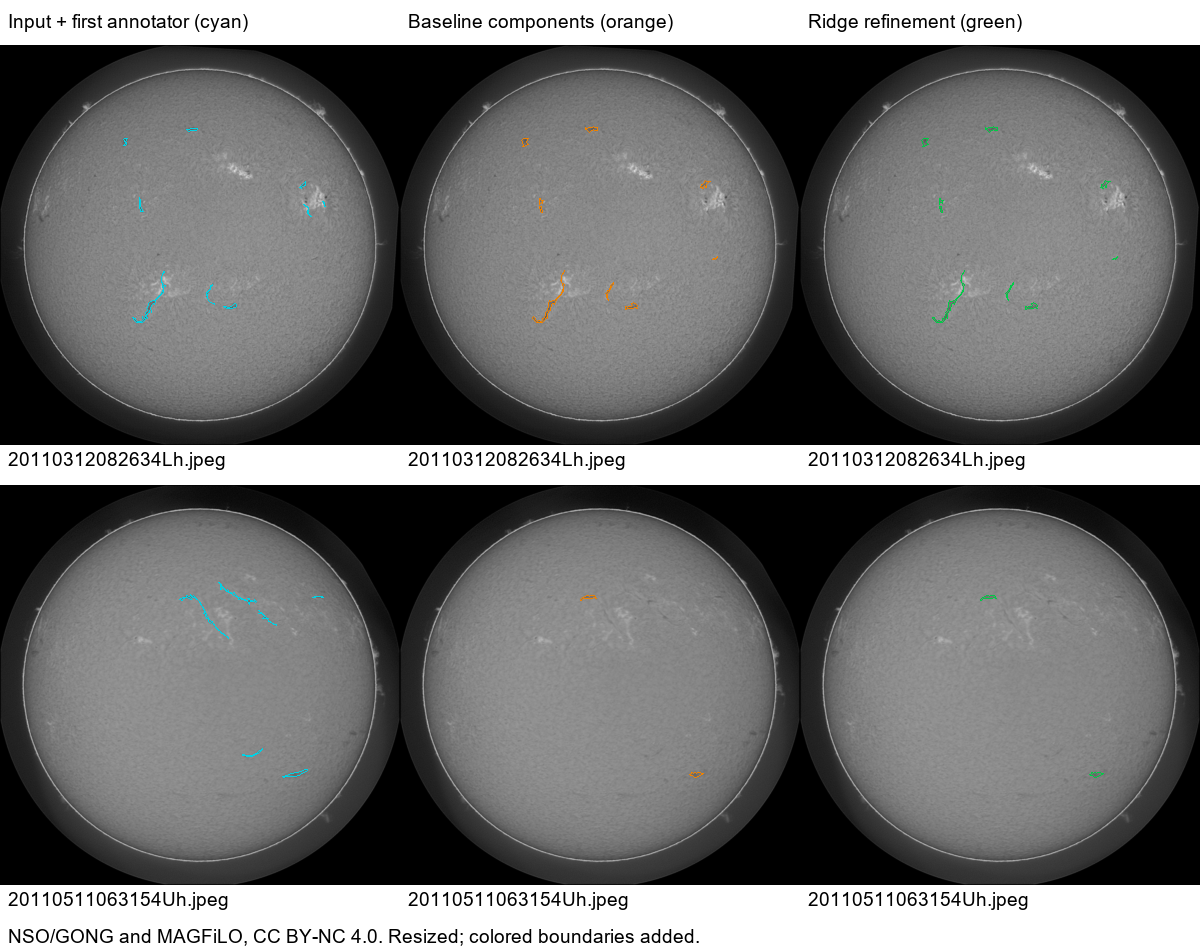
\includegraphics[width=.94\textwidth]{segmentation-examples.png}
\caption{First two filenames in the frozen original assessment list, without outcome-based replacement. Left: image with the first available annotator's boundaries. Middle: component-filter baseline. Right: ridge refinement. These full-disk views are descriptive illustrations, not evidence of a new independent gain. NSO/GONG and MAGFiLO, CC BY-NC 4.0; resized with colored boundaries.}\label{fig:examples}\end{figure*}
\subsection{What changes and what does not}
On the first comparison, TP increases from 445 to 447 and FN falls from 682 to 680. On the additional 40 images, TP increases from 224 to 225 and FN falls from 300 to 299, but thin TP stays at 44. Combined TP is 669 versus 672, FN 982 versus 979. The net thin gain is one annotation-level match among 442 thin annotations; this is a modest, unstable effect rather than robust thin-filament recovery.

Descriptive paired date-bootstrap 95\% intervals for PQ gain are $[-0.001377,0.004161]$ on the first set and $[-0.000574,0.003717]$ on the additional set. Both contain zero. The combined result is a descriptive aggregation of two reused comparisons, not a third independent trial. The additional set fails the criterion requiring a strict gain in thin matches, even though overall PQ and FP improve slightly. We retain this negative result.

Fragmentation/merging also remain unresolved. Combined diagnostic split counts are 150 for both methods and merge counts six for both. The first set has 95 split and five merge counts under each method; the additional set has 55 and one. These diagnostics depend on the public mask-overlap definitions and do not count unique physical structures. Ridge trimming does not repair a fundamentally missing or incorrectly grouped component.
\subsection{Failed alternatives and practical limits}
Earlier proposal-based thin-component filtering reproduced baseline thin matches (82/314) and 550 FP exactly. A joint rejection variant reduced FP to 546 but also reduced TP to 439 and did not add thin matches; it was rejected. Morphological growth, erosion and mask substitution did not satisfy the tuning constraints. The archive preserves these outcomes instead of reporting only the selected model.

The images in Figure~\ref{fig:examples} show how a CPU mask pipeline can be inspected against one annotator, but annotator disagreement, observing conditions and downsampling remain important limitations. Full-disk visual similarity is not a substitute for the numerical comparisons. A substantially better future method would need independently measured sensitivity to previously missing fine structures, while controlling extra detections on genuinely new dates.

\section{Reproduction and candidate update}
\subsection{Code, dependencies and a fresh-copy audit}
The public source release is pinned at Solar repository commit \texttt{7193ec2}; the full digest and reproducibility links accompany this local update. Commands run from \texttt{releases/2026-10-16/}. Python 3.12 dependencies are NumPy 2.5.4, SciPy 1.18.1, Pillow 12.3.0, pycocotools 2.0.11, scikit-learn 1.7.2, joblib 1.5.2, threadpoolctl 3.6.0 and pytest 8.4.2. Torch is unnecessary for this candidate. Source, model and frozen-protocol digests are checked before image-only inference.

A fresh GitHub clone and a new isolated environment installed those requirements without dependency conflicts. All six package tests passed; prediction exactly reproduced the recorded label-array SHA-256 for image \texttt{20110621063134Lh.jpeg}. A new training workspace also imported the unchanged scripts, verified the annotation hash, decoded one training image and produced finite baseline $(1024,1024,24)$ and ridge $(2048,2048,10)$ feature arrays. Full training was not repeated during this audit, so it does not prove byte-identical model serialization across environments.

\subsection{New local CSV and verification}
The new candidate runs the frozen three-model image-only pipeline on all 180 test observations. It contains 1136 predicted instances and 11 images with no instance rows. Each exported COCO RLE is decoded and compared with its exact predicted mask. An independent audit verifies the two-column schema, unique image/object identifiers, contiguous local suffixes, image registry, input hashes and non-overlapping masks. Zero detections create zero object rows, rather than a fabricated placeholder. This follows the inspected public evaluator; private upload validation remains untested.

This candidate has no Kaggle score yet. The earlier entry's reported 0.14 score belongs to a different model and CSV and cannot be attached to this new file. The CSV has not been uploaded to Kaggle; publishing a report on GitHub does not submit the entry. The exact candidate digest, counts and file sizes are in the accompanying manifest. A future organizer-form update must attach exactly the same CSV as the one accepted by Kaggle, not a different local export.

\subsection{Complete exact-inference materials}
This update supplies the exact three fitted joblib models, verified digests, whole-test-set exporter and full-pipeline notebook under \texttt{submission-update-2026-10-16/}. The original source-only release remains unchanged. A fresh clone needs only the separately obtained authorized test images, pinned Python dependencies and these public materials; it does not need a private weight folder, training annotations or paid inference. The notebook's full-export cell regenerates all 180 predictions and checks the frozen CSV digest.

The reference CSV SHA-256 is \texttt{9d8f64cdca2fcf99}\linebreak\texttt{6ca8efefff5f6444}\linebreak\texttt{ecee1480195ddb31}\linebreak\texttt{2a8e72029e63a639} (four concatenated segments). The public verification record documents the clean-copy run and independent mask/schema/input checks. Data-derived fitted models and example graphics are marked CC BY-NC 4.0 with NSO/GONG and MAGFiLO attribution; original code remains Apache-2.0. No original observation or annotation archive is redistributed. Full retraining remains optional and was not repeated for this exact-inference update.

\section*{Acknowledgment}
The organization of the Filament Segmentation Challenge 2026 is partially supported by the U.S. National Science Foundation (NSF) under Grant No. 2209912 and 2433781, directorate for Computer and Information Science and Engineering (CSE), and Office of Advanced Cyberinfrastructure (OAC), and Grant No. 2511630, AST Division Of Astronomical Sciences and MPS Directorate for Mathematical and Physical Sciences. The Filament Segmentation Challenge 2026 is sponsored by the U.S. National Science Foundation (NSF) National Solar Observatory (NSO). This work utilizes GONG data obtained by the NSO Integrated Synoptic Program, managed by the National Solar Observatory, which is operated by the Association of Universities for Research in Astronomy (AURA), Inc. under a cooperative agreement with the National Science Foundation and with contribution from the National Oceanic and Atmospheric Administration. The GONG network of instruments is hosted by the Big Bear Solar Observatory, High Altitude Observatory, Learmonth Solar Observatory, Udaipur Solar Observatory, Instituto de Astrofísica de Canarias, and Cerro Tololo Interamerican Observatory.
\section*{References}
\begingroup\raggedright\small
[1] Ahmadzadeh et al. Solar Filament Segmentation Challenge 2026. Kaggle. \url{https://www.kaggle.com/competitions/filament-segmentation-2026}.

[2] Ahmadzadeh et al. A dataset of manually annotated filaments from H-alpha observations. Scientific Data 11, 1031 (2024). \url{https://doi.org/10.1038/s41597-024-03876-y}.

[3] Ahmadzadeh. Self-Evaluation Notebook, public v6. \url{https://www.kaggle.com/code/azimahmadzadeh/self-evaluation-notebook}. Inspected study artifact and organizer overview, 16 October 2026.

[4] Geurts, Ernst and Wehenkel. Extremely randomized trees. Machine Learning 63, 3--42 (2006). \url{https://doi.org/10.1007/s10994-006-6226-1}.

[5] Jacek Adamek. ThreadMask source release, 16 October 2026. \href{https://github.com/jacman1988-super/solar-threadmask/tree/7193ec292d0dee31993c5bd23e013ea49ffdc981/releases/2026-10-16}{Source release at commit 7193ec2}.
\endgroup
\end{document}
